%%%%%%%%%%%%%%%%%%%%%%%%%%%%%%%%%%%%%%%%%%%%%%%%%%%%%%%%%%%%%%%%
%                                                              %
%                                                              %
% Macallyster S. Edmondson                                     %
%                                                              %
% ECE351-53                                                    %
%                                                              %
% Lab #10                                                      %
%                                                              %
% 04/05/2022                                                   %
%                                                              %
% Straightforward layout, broken into sections, uses many      %
% common libraries. Note, Hyperlinks are not highlighted.      %
%                                                              %
%%%%%%%%%%%%%%%%%%%%%%%%%%%%%%%%%%%%%%%%%%%%%%%%%%%%%%%%%%%%%%%%

%%%%%%%%%%%%%%%%%%%%%%%%%%%%%%%%%%%%%%%%%%%
%%% DOCUMENT PREAMBLE %%%
\documentclass[12pt]{report}
\usepackage[english]{babel}
%\usepackage{natbib}
\usepackage{url}
\usepackage[utf8x]{inputenc}
\usepackage{amsmath}
\usepackage{graphicx}
\graphicspath{{./images/}}
\usepackage{parskip}
\usepackage{fancyhdr}
\usepackage{vmargin}
\usepackage{listings}
\usepackage[hidelinks]{hyperref}
\usepackage{xcolor}
\usepackage[nodayofweek]{datetime}
\usepackage[section]{placeins}
\usepackage{pdfpages}
\usepackage{float}
\definecolor{codegreen}{rgb}{0,0.6,0}
\definecolor{codegray}{rgb}{0.5,0.5,0.5}
\definecolor{codeblue}{rgb}{0,0,0.95}
\definecolor{backcolour}{rgb}{0.95,0.95,0.92}
\lstdefinestyle{mystyle}{
backgroundcolor=\color{backcolour},
commentstyle=\color{codegreen},
keywordstyle=\color{codeblue},
numberstyle=\tiny\color{codegray},
stringstyle=\color{codegreen},
basicstyle=\ttfamily\footnotesize,
breakatwhitespace=false,
breaklines=true,
captionpos=b,
keepspaces=true,
numbers=left,
numbersep=5pt,
showspaces=false,
showstringspaces=false,
showtabs=false,
tabsize=2
}
\lstset{style=mystyle}
\setmarginsrb{3 cm}{2.5 cm}{3 cm}{2.5 cm}{1 cm}{1 cm}{1 cm}{1.5 cm}
\title{Lab \#10 Report}
% Title
\author{Macallyster S. Edmondson}
% Author
\newdate{date}{05}{04}{2022}
\date{\longdate\displaydate{date}}
% Date
\makeatletter
\let\thetitle\@title
\let\theauthor\@author
\let\thedate\@date
\makeatother
\pagestyle{fancy}
\fancyhf{}
\rhead{\theauthor}
\lhead{\thetitle}
\lfoot{Page: \thepage}
\rfoot{\thedate}
\fancypagestyle{customplain}{ %Used for default pages with plain style to keep overall document consistency
  \fancyhf{}
  \renewcommand{\headrulewidth}{0pt} %Remove bar from top of page
  \lfoot{Page: \thepage}
}
\fancypagestyle{titlepage}{ %Used for default pages with plain style to keep overall document consistency
  \fancyhf{}
  \renewcommand{\headrulewidth}{0pt} %Remove bar from top of page
  \cfoot{\thedate}
}
\fancypagestyle{customblank}{ %Used for default pages with plain style to keep overall document consistency
  \fancyhf{}
  \renewcommand{\headrulewidth}{0pt} %Remove bar from top of page
}
%%%%%%%%%%%%%%%%%%%%%%%%%%%%%%%%%%%%%%%%%%%%
\begin{document}
%%%%%%%%%%%%%%%%%%%%%%%%%%%%%%%%%%%%%%%%%%%%%%%%%%%%%%%%%%%%%%%%%%%%%%%%%%
%%%%%%%%%%%%%%%
\begin{titlepage}\thispagestyle{titlepage}
\centering
%\vspace*{0.5 cm}

\includegraphics[scale = 0.12]{univ-logo.png}\\[1.0 cm]
%University of Idaho
\begin{center}    \textsc{\Large   ECE 351 - Section \#53 }\\[2.0 cm]
\end{center}% University Name

%Lab Report
\rule{\linewidth}{0.2 mm} \\[0.4 cm]
{ \huge \bfseries \thetitle}\\
\rule{\linewidth}{0.2 mm} \\[0.5 cm]
\textsc{\Large Frequency Response }\\[1.5 cm] % Course 
\begin{minipage}{0.4\textwidth}
\begin{flushleft} \large
\emph{Submitted To:}\\
Kate Antonov\\ \small
University of Idaho\\
kantonov@uidaho.edu\\
\hfill
\end{flushleft}
\end{minipage}~
\begin{minipage}{0.4\textwidth}
\begin{flushright} \large
\emph{Submitted By :} \\
\theauthor \\ \small
University of Idaho\\
edmo7033@vandals.uidaho.edu\\
\href{http://github.com/mac-edmondson}{github.com/mac-edmondson}\\
\end{flushright}
\end{minipage}\\[2 cm]
\vfill
\end{titlepage}
%%%%%%%%%%%%%%%%%%%%%%%%%%%%%%%%%%%%%%%%%%%%%%%%%%%%%%%%%%%%%%%%%%%%%%%%%%
%%%%%%%%%%%%%%%
\tableofcontents\thispagestyle{customplain}
\pagebreak
%%%%%%%%%%%%%%%%%%%%%%%%%%%%%%%%%%%%%%%%%%%%%%%%%%%%%%%%%%%%%%%%%%%%%%%%%%
%%%%%%%%%%%%%%%
\renewcommand{\thesection}{\arabic{section}}
\section{Introduction}
The goal of this weeks lab was to become familiar with frequency response tools and Bode plots using Python.
This lab was completed using\textit{Python} through the \textit{Spyder-IDE}. The packages used in the completion 
of this lab were \texttt{numpy} for definitions of mathematical functions, \texttt{matplotlib.pyplot} to plot outputs 
of functions, \texttt{scipy.signal} to filter an input based on a transfer function, and \texttt{control} to create
Bode plots with already existing functions.

All code for this lab, including this report, can be found on \href{http://github.com/mac-edmondson}{my Github}.
\section{Equations}\label{section: eq}
The equations used within this lab are shown in this section. The equations will be referenced by number throughout
the rest of the report.

Preliminary Transfer Function \& derived magnitude and phase:
\begin{equation}\label{eq: cirTF} %Full Fourier Series
  \begin{aligned}[c]
    H(s) = \frac{\frac{1}{RC}s}{s^2 + \frac{1}{RC}s + \frac{1}{LC}} 
  \end{aligned}
\end{equation}
\begin{equation}\label{eq: cirTFmag}
  \begin{aligned}[c]
    |H(j\omega)| = \frac{\frac{1}{RC}\omega}{\sqrt{\omega^4 + [(\frac{1}{RC})^2 - \frac{2}{LC}]\omega^2 + (\frac{1}{LC})^2}}
  \end{aligned}
\end{equation}
\begin{equation}\label{eq: cirTFang}
  \begin{aligned}[c]
    \angle H(j\omega) = \frac{\pi}{2} - \tan^{-1}{(\frac{\frac{1}{RC}\omega}{-\omega^2 + \frac{1}{LC}})}
  \end{aligned}
\end{equation}
Part 2 Input Signal:
\begin{equation}\label{eq: inForFilter}
  \begin{aligned}[c]
    x(t) = \cos{(2\pi\cdot 100t)} + \cos{(2\pi\cdot 3024t)} + \sin(2\pi\cdot 50000t)
  \end{aligned}
\end{equation}

\section{Methodology}
\subsection{Lab: Part 1}\label{Section: Part1}
In Part 1 of this lab, we used the derived magnitude and angle of the pre-lab [Equations \eqref{eq: cirTFmag} \& \eqref{eq: cirTFang}] to plot a 
Bode plot using the \texttt{matplotlib.pyplot,semilogx()} function. This same process was done using the \texttt{control.bode()} function by simply
plugging in the original transfer function coefficients. One plot was generated with an x-axis unit of Hz which proved quite useful for analysis of
Part 2 of this lab.

Code implementing Part 1 of this lab can be seen in the below listing.

\begin{lstlisting}[language=Python, basicstyle=\footnotesize]
# PART 1

R = 1e3 # Ohms
L = 27e-3 # H
C = 100e-9 # F

# 1
def mag_db(omega) :
    out = (((1/(R*C))*omega)/(np.sqrt((w**4) + ((((1/(R*C))**2) - (2/(L*C))) * (omega**2)) + ((1/(L*C))**2))))
    out_db = 20 * np.log10(out)
    return out_db

def ang_deg(omega) :
    ang = np.pi/2 - np.arctan(((1/(R*C))*omega)/((1/(L*C))-(omega**2)))
    ang_deg = (180/np.pi) * ang
    return ang_deg

w = np.arange(1e3, 1e6 + step_size, step_size)
mag = mag_db(w)
ang = ang_deg(w)

for i in range(len(ang)):
    if(ang[i] > 90):
        ang[i] -= 180

plt.figure(figsize = (10, 11))
plt.subplot(2, 1, 1)
plt.semilogx(w, mag, "b-")
plt.grid(True, which='both', ls='-')
plt.ylabel('|H(S)| [dB]')
plt.title('Magnitude and Phase Bode Plot [Manual]')
plt.subplot(2, 1, 2)
plt.grid(True, which='both', ls='-')
plt.semilogx(w, ang, "b-")
plt.ylabel('angle(H(S)) [deg]')
plt.xlabel('w [rad/s]')

# 2
num = [1/(R*C), 0]
den = [1, 1/(R*C), 1/(L*C)]

sys = con.TransferFunction(num, den)

plt.figure(figsize=(10,11))
plt.title('Magnitude and Phase Bode Plot [spsig.bode]')
_ = con.bode(sys, omega=None, dB = True, Hz = False, deg = True, Plot = True)

plt.figure(figsize=(10, 11))
plt.title('Magnitude and Phase Bode Plot [spsig.bode] (Hz)')
_ = con.bode(sys, omega=None, dB = True, Hz = True, deg = True, Plot = True)
\end{lstlisting}

\subsection{Lab: Part 2}\label{Section: part2}
In Part 2 of this lab we used the \texttt{scipy.signal.bilinear()} \& \\\texttt{scipy.signal.lfilter()} functions to filter the 
input function seen in Equation \eqref{eq: inForFilter}. Figures \ref{fig: p2t1} \& \ref{fig: p2t2} show the input function \textit{x(t)}
and the output after it was run through the filter. This was an extremely useful exercise which I found crucial for my understanding
of concepts discussed in class. Such a simple exercise can be so helpful.

Code implementing Part 2 of this lab can be seen in the below listing.

\begin{lstlisting}[language=Python, basicstyle=\footnotesize]
# PART 2
fs = 2*np.pi*50000
step_size = 1/fs

t = np.arange(0, 0.01 + step_size, step_size)
x = np.cos(2*np.pi*100*t) + np.cos(2*np.pi*3024*t) + np.sin(2*np.pi*50000*t)
plt.figure(figsize=(10, 11))
plt.subplot(1, 1, 1)
plt.plot(t, x, "b-")
plt.grid()
plt.ylabel('x(t)')
plt.xlabel('t')
plt.title('Part 2 Task 1')

z, p= spsig.bilinear(num, den, fs=fs)
y = spsig.lfilter(z, p, x)

plt.figure(figsize=(10, 11))
plt.subplot(1, 1, 1)
plt.plot(t, y, "b-")
plt.grid()
plt.ylabel('y(t)')
plt.xlabel('t')
plt.title('Part 2 Task 4')
\end{lstlisting}

\section{Results}\label{section: Results}
The results of this lab are very straightforward. The implementation of all functions worked as expected and the results are as expected.
More analysis of theory and results is discussed in the \nameref{section: Questions} Section of this report.

The deliverables for Part 1 \& 2 of this lab are seen in all figures given below.
\\
\begin{figure}[h!]
  \centering
  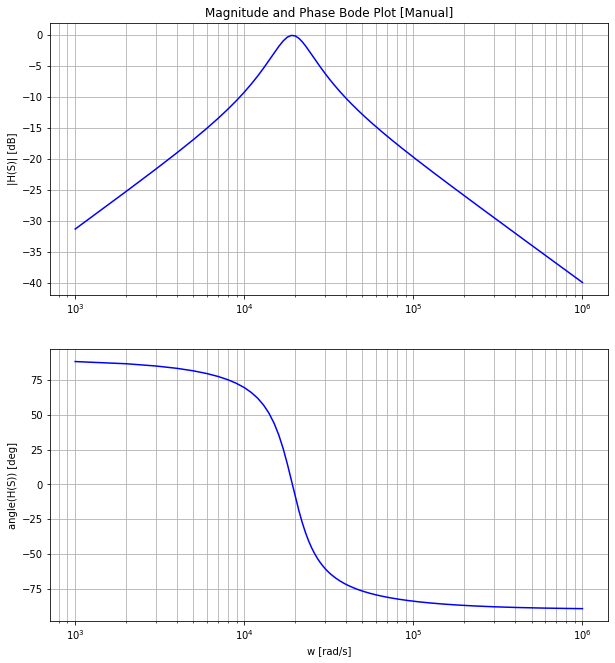
\includegraphics[width=\linewidth]{p1t1.png}
  \caption{Mag. \& Phase Bode Plot, Manual (rad/s) [Equations \eqref{eq: cirTFmag} \& \eqref{eq: cirTFang}]}
  \label{fig: p1t1}
\end{figure}
\begin{figure}[h!]
  \centering
  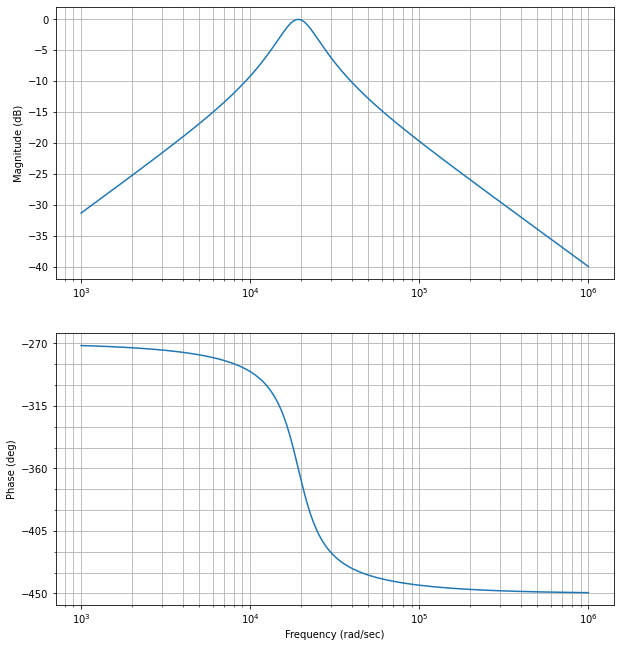
\includegraphics[width=\linewidth]{p1t2.png}
  \caption{Mag. \& Phase Bode Plot, \texttt{spsig.bode()} (rad/s) [Equation \eqref{eq: cirTF}]}
  \label{fig: p1t2}
\end{figure}
\begin{figure}[h!]
  \centering
  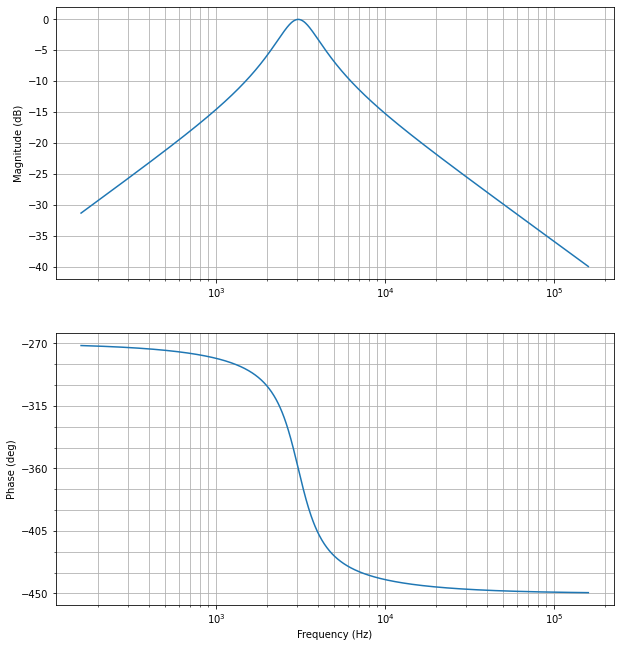
\includegraphics[width=\linewidth]{p1t3.png}
  \caption{Mag. \& Phase Bode Plot, \texttt{spsig.bode()} (Hz) [Equation \eqref{eq: cirTF}]}
  \label{fig: p1t3}
\end{figure}
\begin{figure}[h!]
  \centering
  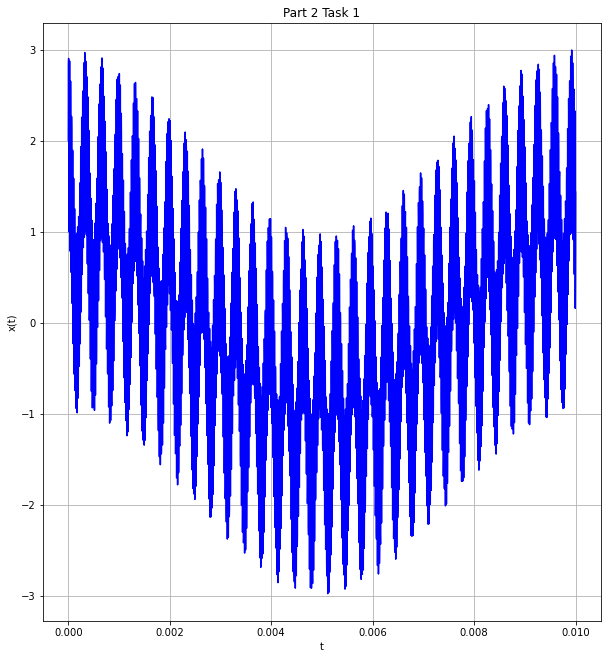
\includegraphics[width=\linewidth]{p2t1.png}
  \caption{Filter Input Function, x(t)  [Equation \eqref{eq: inForFilter}]}
  \label{fig: p2t1}
\end{figure}
\begin{figure}[h!]
  \centering
  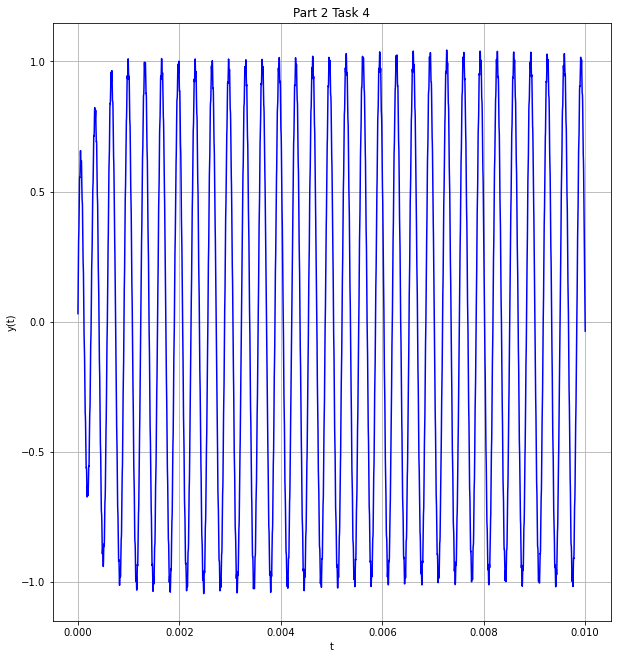
\includegraphics[width=\linewidth]{p2t2.png}
  \caption{Filter Output}
  \label{fig: p2t2}
\end{figure}


\section{Error Analysis}\label{section: ErAn}
No sources of error were seen throughout this lab other than the need for a phase shift of the manually plotted Bode plot (Figure \ref{fig: p1t1}) for readability purposes.
Other than this no other issues were encountered.
\section{Questions}\label{section: Questions}
\begin{enumerate}
  \item Explain how the filter and filtered output in Part 2 makes sense given the Bode plots from Part 1. Discuss how the filter modifies specific frequency bands, in Hz.
  \begin{itemize}
    \item As seen from the Bode plots in Part 1, the filter described by the transfer function is a band-pass filter only allowing frequencies of ~2e4 rad/s (~ 3e3 Hz) through.
    Thus the dominant term that should be seen in the output of the filter should be the second term from the input, Equation \eqref{eq: inForFilter}.
    Looking at the plot in Figure \ref{fig: p2t2}, we can see there are approximately 6 periods in 2 milliseconds which gives an approximate frequency of 3000 Hz.
    As this is the frequency of the second term in the input signal, it appears the filter is working properly. As the frequency is not exactly 3000 Hz, the
    output of the filter will have a slight magnitude attenuation and phase shift (more noticeable) which is seen in the output of the filter, Figure \ref{fig: p2t2}. 
  \end{itemize}
  \item Discuss the purpose and workings of \\\texttt{scipy.signal.bilinear()} and \texttt{scipy.signal.lfilter()}.
  \begin{itemize}
    \item The \texttt{spsig.bilinear()} function performs a bilinear transformation on an s-domain transfer function into the z-domain using Tustin's method.
    Once the transfer function is in the z-domain, digital filtering is much easier to achieve. The z-domain filter is then plugged into the \\\texttt{spsig.lfilter()}
    function which uses the z-domain to filter the input function, then is transformed back and returned.
  \end{itemize}
  \item What happens if you use a different sampling frequency in \\\texttt{scipy.signal.bilinear()} than you used for the time-domain signal?
  \begin{itemize}
    \item Like seen in Lab \#9, a different frequency sample could have detrimental consequences. If a frequency sample close to the time-domain
    sampling frequency is used, the output will look close to what it should be but could be time shifted and scaled slightly. If a vastly different
    sampling frequency is used, the output will unrecognizable due to the amount of time scaling that takes place. In either case, the results of
    the output function will be incorrect.
  \end{itemize}
  \item Leave any feedback on the clarity of lab tasks, expectations, and deliverables.
  \begin{itemize}
    \item This lab was very clear for all instructions, expectations and deliverables.
  \end{itemize}
\end{enumerate}
\section{Conclusion}
In conclusion, I feel this lab was very successful. I really enjoyed the lab questions which helped me recognize some aspects of filters I did not understand before.
I feel this has been one of the most helpful labs for my understanding of class topics. All in all, I am very satisfied with what this lab has taught me and feel it was an 
excellent use of time.
\newpage
\thispagestyle{customblank}
\section{Attachments}\label{section: Attachments}
\centering\begin{enumerate}
  \item Pre-Lab
\end{enumerate}
\vspace*{\fill}

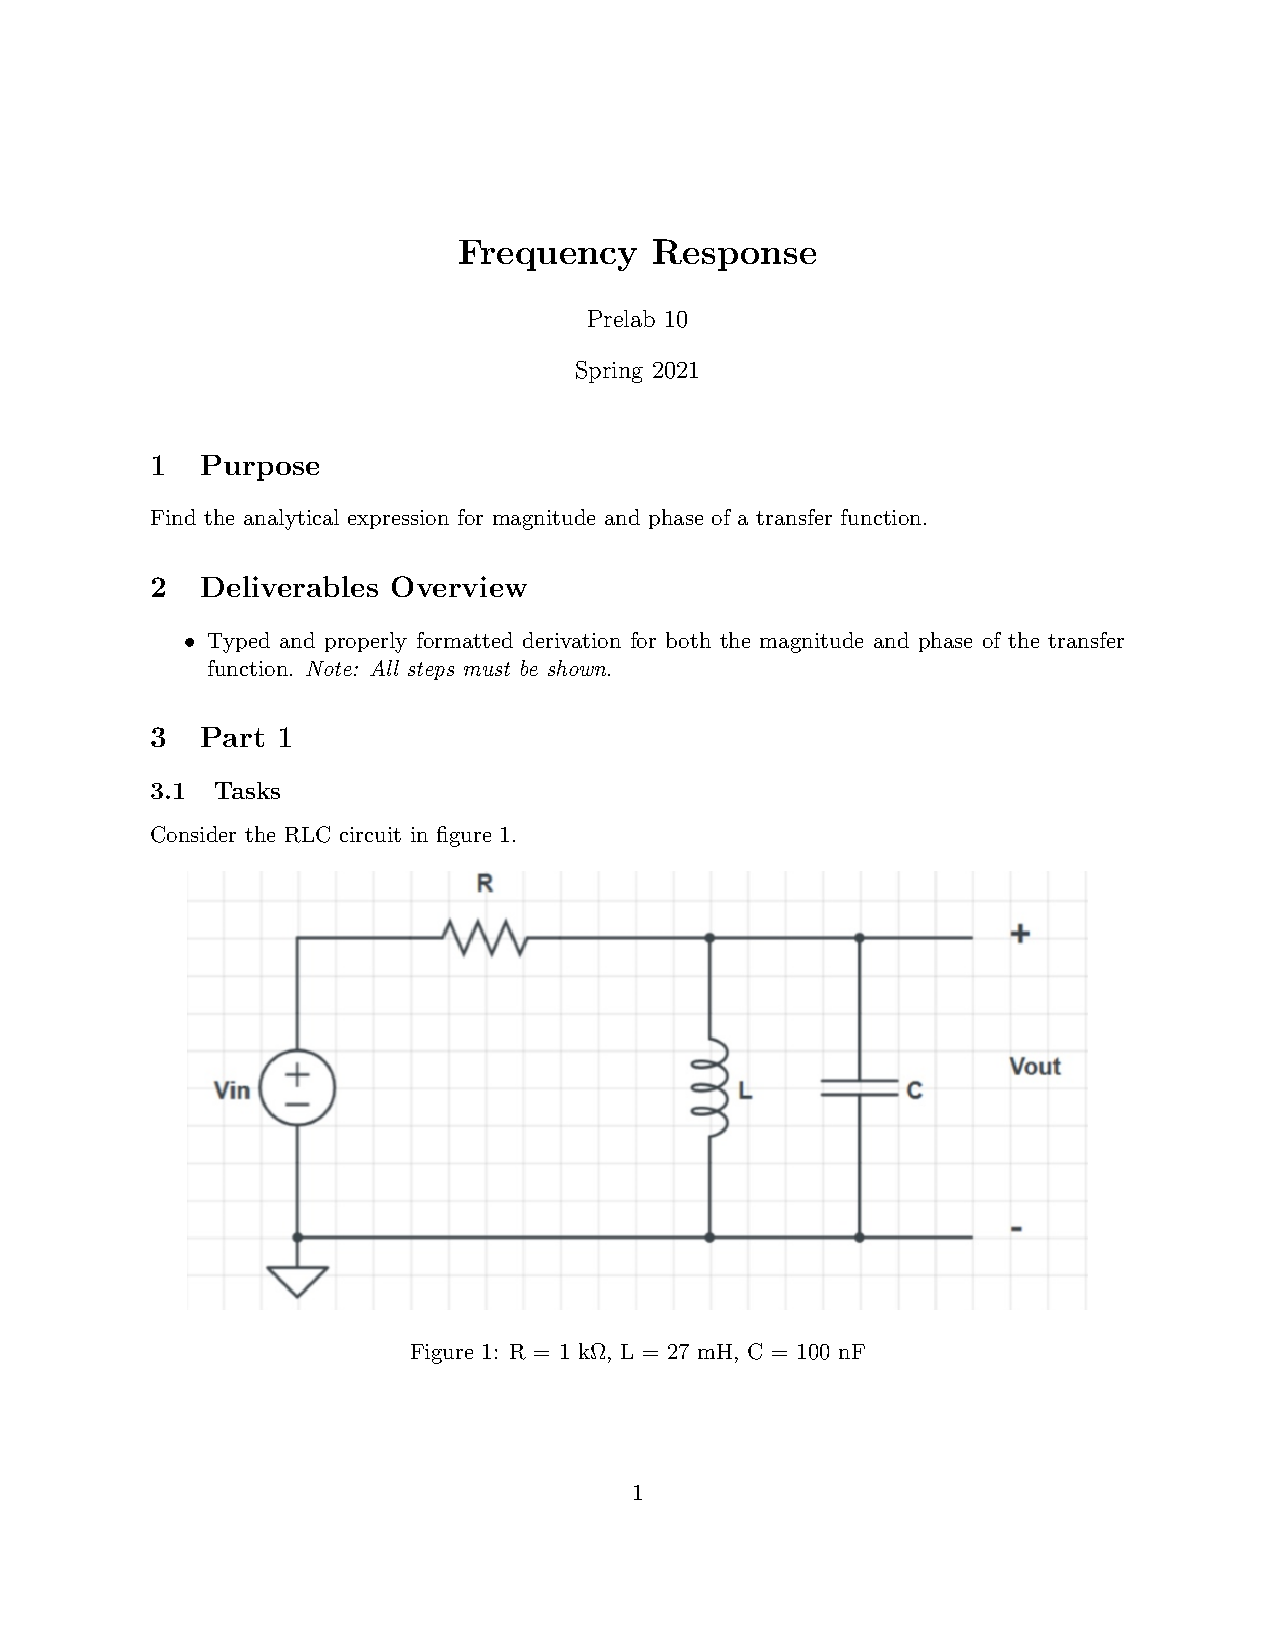
\includepdf[pages=-, offset=1in -1in]{./attachments/lab10_pre.pdf}
% \includepdf[pages=3, offset=1in -1in]{./attachments/lab5.pdf}

% \begin{thebibliography}{111} 
% \thispagestyle{customplain}

% \end{thebibliography}
\end{document}
%This template was created by Roza Aceska.